\documentclass[../compilation_of_summaries/all_summaries.tex]{subfiles}
\begin{document}
	The paper \cite{Balagadde2008} describes the synthetic construction of a predator prey system composed of two engineered E. coli microbes. Through introducing two quorum sensing (cell density sensing) modules from Vibrio fischeri (the LuxI/LuxR genes) and Pseudomonas aeruginosa (the LasI/LasR genes) the authors are able to construct a predator E. coli which grows at the cost of the prey E. coli. The predator microbe naturally produces a suicide protein (ccdB) which is inhibited (the antidote ccdA is promoted in the predator) by the expression of a the LuxI gene in the prey. Thus higher cell densities of the prey lead to higher cell densities of the predator. However, the predator cells express the LasI gene which promote the expression of the suicide gene in the prey microbes. This interaction is communicated through acyl-homoserine lacton; see figure \ref{fig:balagadde2008_predprey}.  
	\begin{figure}[h]
		\centering
		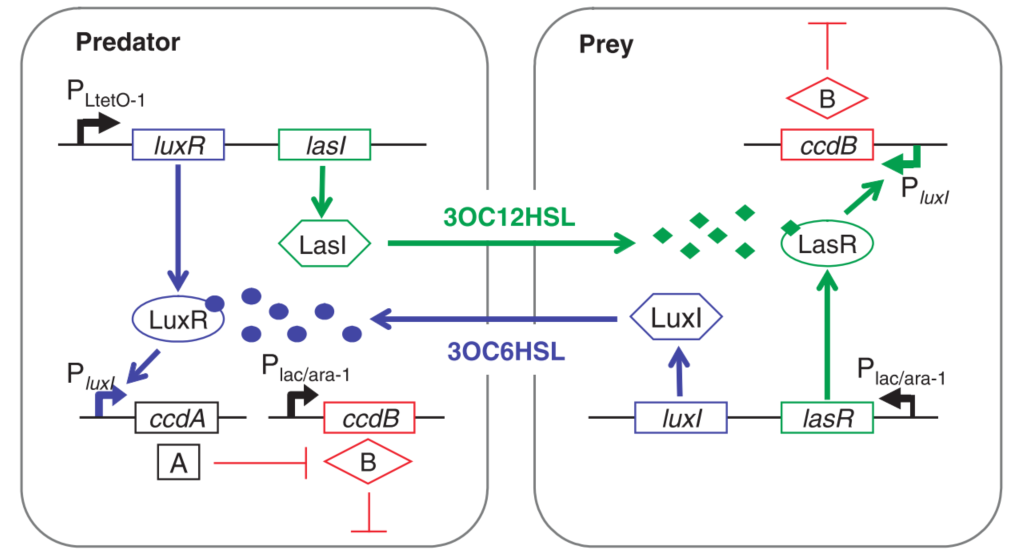
\includegraphics[width=0.8\textwidth]{balagadde2008_predprey.png}
		\caption{Predator Prey gene circuits.}
		\label{fig:balagadde2008_predprey}
	\end{figure}
	The gene circuits were used to model coupled ODEs describing the interacting system (the standard predator prey model). It was reported that this was one of the most complicated synthetic systems studied to date (2008). The authors report that long term characterization, which is essential to verification of the designed circuits is challenging. The authors used a microchemostat to slow down bacterial evolution and stabilize bacterial population size to aid long term culturing. The authors noted that the system was highly sensitive to external conditions (e.g. the chemostat dilution rate). 
	
\end{document}